\documentclass{beamer}

\usepackage{alltt}%
\usetheme{Boadilla}
\usecolortheme{seahorse}

\usepackage[utf8]{inputenc}
\usepackage{default}

\usepackage{xcolor}%for color mixing

\usepackage{amsmath}%
\usepackage{amsfonts}%
\usepackage{amssymb}%
\usepackage{graphicx}


\setbeamertemplate{itemize/enumerate body begin}{\small}


%%%%%%%%%%%%%%%%%%%%%%%%%%%%%%%%%%%%%%%%%%%%%%%%%%%%%%%%%%%%%%%%%%%%%%%%%%%%%%%%%%

\title{Statisitcal Thinking in Biology Research}
\author{Terry Neeman and Timothee Bonnet}
\date{\today}

\begin{document}

\begin{frame}{}
\maketitle

\end{frame}
%%%%%%%%%%%%%%%%%%%%%%%

\begin{frame}{Acknowledgemnts and warning}

\end{frame}
%%%%%%%%%%%%%%%%%%%%%%%

\begin{frame}{Key ideas for today}

\begin{itemize}[<+->]
 \item Statistics in biology is the study of biological variation
 \item Statistical ideas about biological variation inform the design of experiments
 \item Statistical ideas about biological variation inform the analysis of experiments
 \item Statistical thinking is an essential component of scientific thinking
\end{itemize}

\end{frame}
%%%%%%%%%%%%%%%%%%%%%%%

\begin{frame}{A bit of history of statistical methods}
 
 R.A. Fisher: 1890-1962
 \only<1>{\begin{center}
  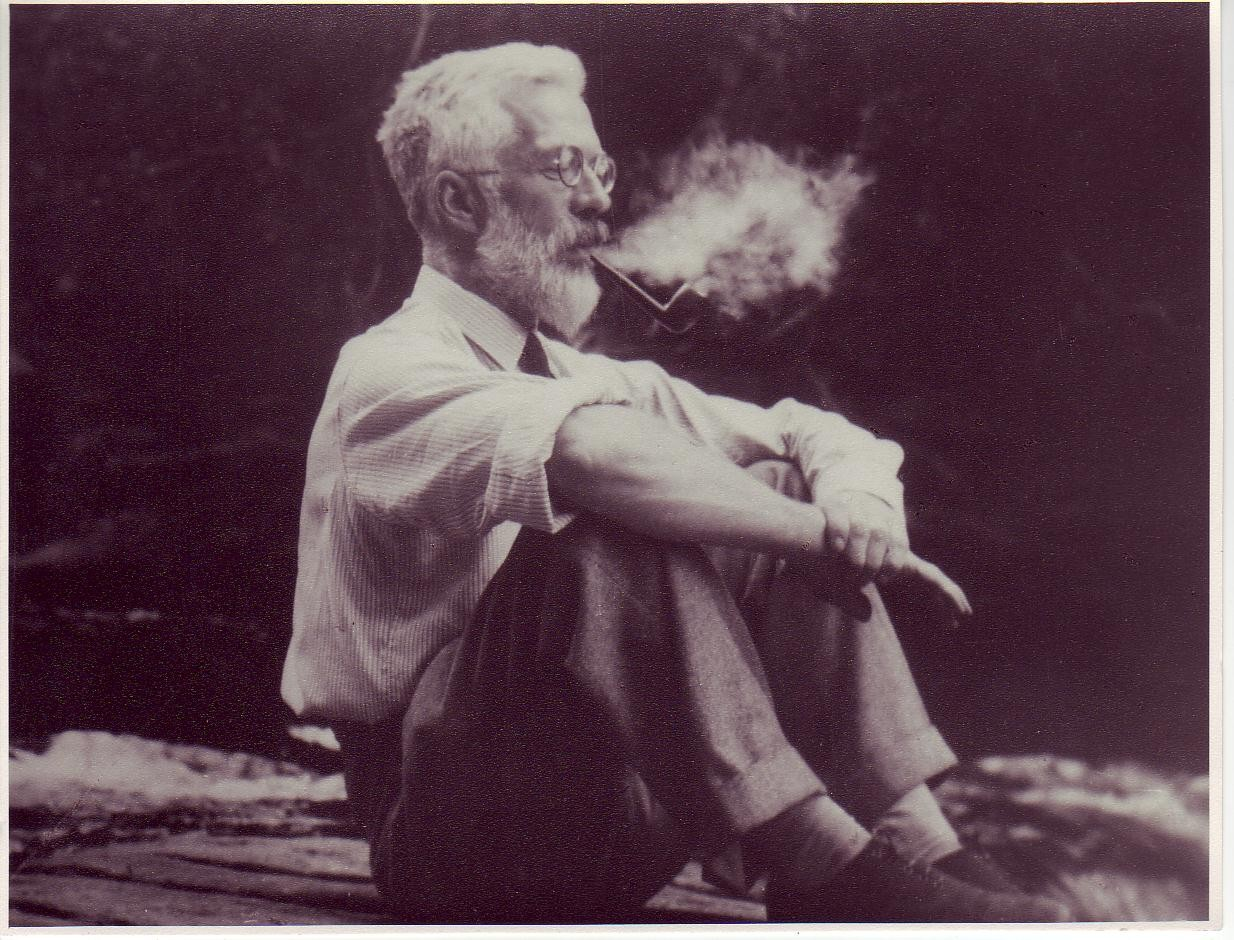
\includegraphics[width=0.5\textwidth]{Figures/fisher}
 \end{center}}
 
 \only<2>{\begin{center}
  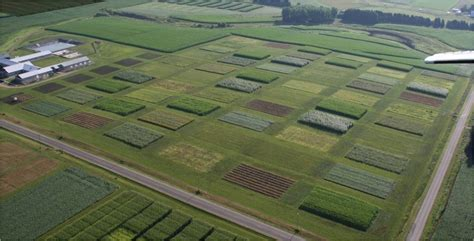
\includegraphics[width=0.9\textwidth]{Figures/fields}
 \end{center}}
 
 Statistical Principles for Research Workers (1925)

\end{frame}
%%%%%%%%%%%%%%%%%%%%%%%

\begin{frame}{Cautionary tales from the front}

\end{frame}
%%%%%%%%%%%%%%%%%%%%%%%

\begin{frame}{Message 1: A small p-value is not always evidence of a treatment effect}

  \begin{columns}
    \begin{column}{0.5\textwidth}
	\begin{center}
	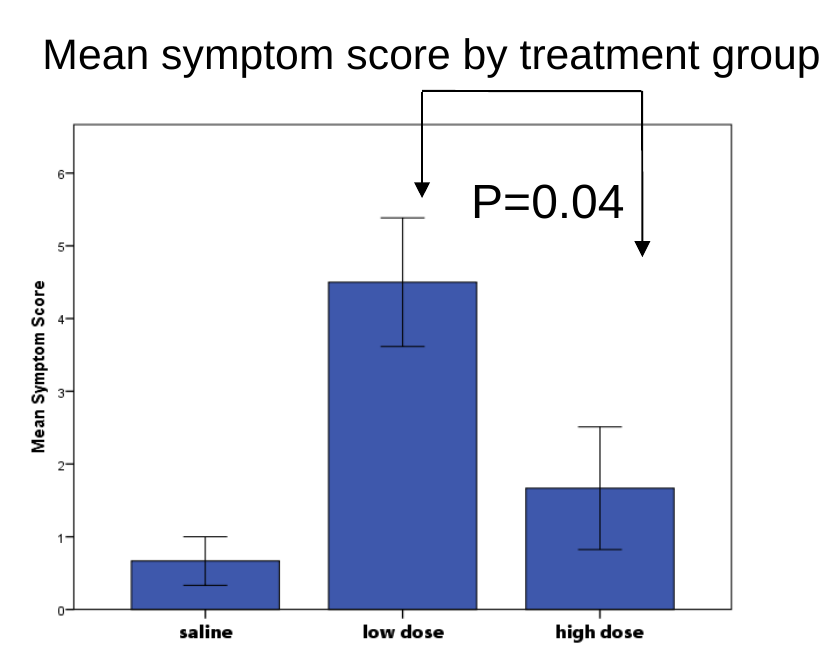
\includegraphics[width=\textwidth]{Figures/message1}
	\end{center}
    \end{column}
    
    \begin{column}{0.5\textwidth}
    \begin{block}{Vaccine challenge experiment:}
      \begin{itemize} 
       \item 6 mice/group (saline/low dose/high dose)
       \item All mice challenged with Shigella
       \item Followed for 14 days
       \item  Outcome: Symptom score average Days 2 - 8
      \end{itemize}
      \end{block}
      
      \begin{alertblock}{}
       One-way ANOVA (post-hoc Bonferroni) p=0.04
      \end{alertblock}

    \end{column}
  \end{columns}
  
  \pause \vspace{0.3cm}
  \emph{\large Do you think the vaccine works? What is strange?}
  

\end{frame}
%%%%%%%%%%%%%%%%%%%%%%%

\begin{frame}{Message 1: A small p-value is not always evidence of a treatment effect}
\pause
 \vspace{-0.2cm}
 \begin{center}
  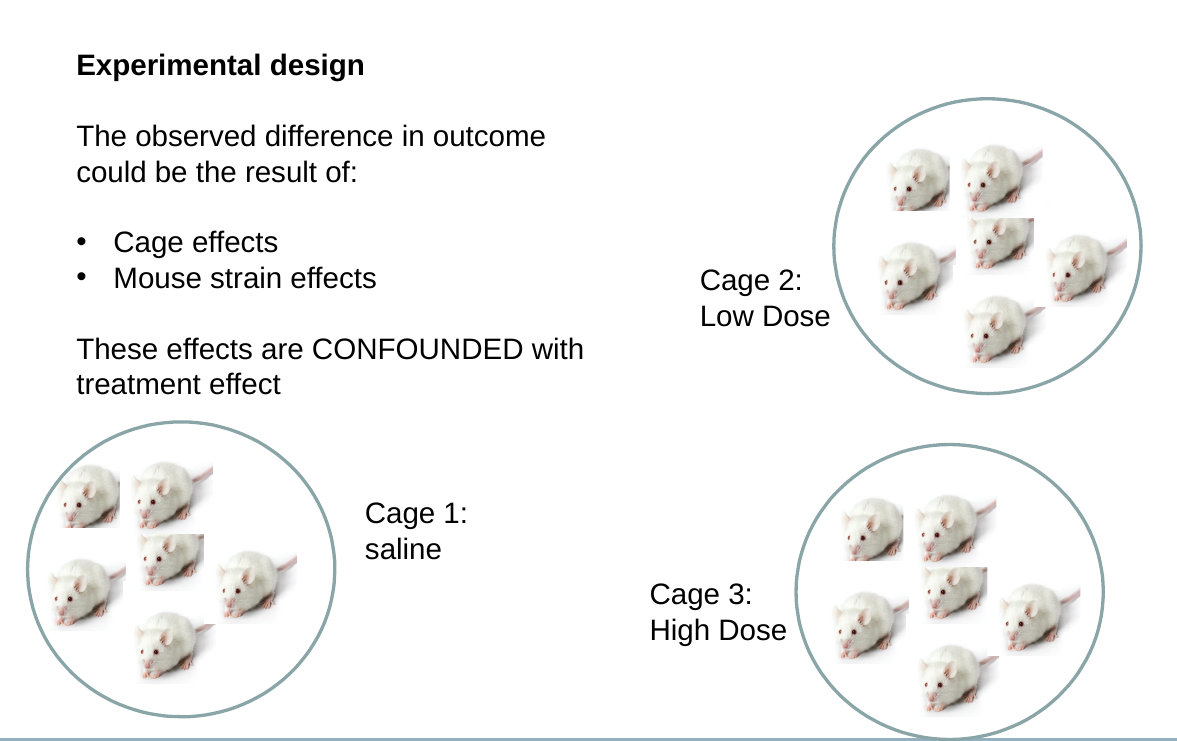
\includegraphics[width=\textwidth]{Figures/mice}
 \end{center}
 
\end{frame}
%%%%%%%%%%%

\begin{frame}{Message 2: p-values from simple comparisons cannot tell us when differences are “different”}
 \pause
  \begin{columns}
    \begin{column}{0.5\textwidth}
	\begin{center}
	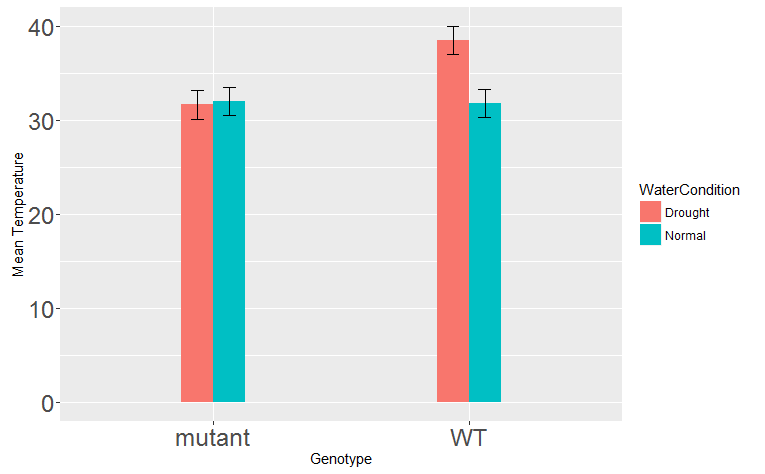
\includegraphics[width=\textwidth]{Figures/message2}
	\end{center}
    \end{column}
    
    \begin{column}{0.5\textwidth}
    \begin{block}{Are temperature mechanisms modified in a genetically modified tomato plant?}
      \begin{itemize}
	\item Genotypes: WT/mutant 
	\item Water condition: Normal/Drought
	\item Leaf temperature measured
      \end{itemize}
      \end{block}
  
    \end{column}
  \end{columns}
   
   
   \begin{alertblock}{Comparisons made using t-tests}
Evidence of difference + No evidence of difference $\neq$ Evidence that differences are different.
      \end{alertblock}
      
      
\end{frame}
%%%%%%%%%%%


\begin{frame}{Message 3: Interpreting experimental results needs more than t-tests}
 \pause
 Research question: Are mice susceptible to obesity when exposed to a high fat diet?
 
  \begin{columns}
    \begin{column}{0.5\textwidth}
	\begin{center}
	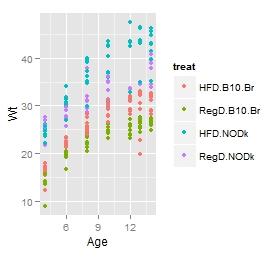
\includegraphics[width=\textwidth]{Figures/message3}
	\end{center}
    \end{column}
    
    \begin{column}{0.5\textwidth}
    \begin{block}{Experimental set-up:}
      \begin{itemize}
	\item 37 mice: 16 NODk /21 WT
	\item Randomised to either regular or high fat diet
	\item Monitored for 14 weeks
	\item Outcome measure: Body weight (g)
	\item Experimental factors: Diet (2), Strain (2), Time (8)
      \end{itemize}
      \end{block}
      \tiny Acknowledgements: Ainy Hussain, PhD student 2013
    \end{column}
  \end{columns}
   
\end{frame}
%%%%%%%%%%%

\begin{frame}{Message 4: Knowing how to combine information across subgroups  can improve inference}
 
 \pause 
 
 Comparing yield in five barley varieties (1930s) \\
 Experimental factors: 5 varieties of barley, 6 locations, 2 time points. Outcome measure: yield
  \begin{columns}
    \begin{column}{0.6\textwidth}
	\begin{center}
	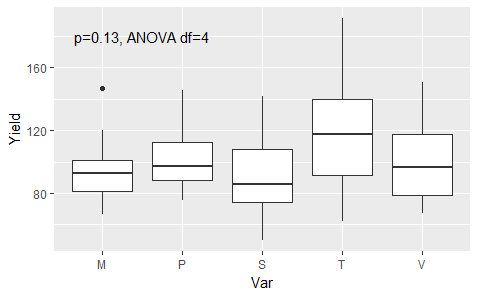
\includegraphics[width=\textwidth]{Figures/message4a}
	\end{center}
    \end{column}
    
    \begin{column}{0.4\textwidth}
  
    \end{column}
  \end{columns}
      \tiny Acknowledgements: MASS R-package
   
\end{frame}
%%%%%%%%%%%


\begin{frame}{Message 4: Knowing how to combine information across subgroups  can improve inference}
 
  
 Comparing yield in five barley varieties (1930s) \\
 Experimental factors: 5 varieties of barley, 6 locations, 2 time points. Outcome measure: yield
  \begin{columns}
    \begin{column}{0.5\textwidth}
	\begin{center}
	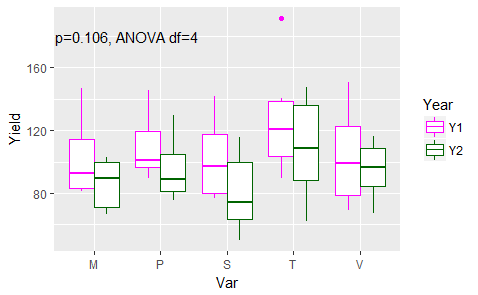
\includegraphics[width=\textwidth]{Figures/message4b}
	\end{center}
    \end{column}
    
    \begin{column}{0.5\textwidth}
    \begin{block}{Controlling for other sources of variation:}
      \begin{itemize}
	\item Controlling for year = comparing yield WITHIN years and combining these
      \end{itemize}
      \end{block}
      \tiny Acknowledgements: MASS R-package
    \end{column}
  \end{columns}
   
\end{frame}
%%%%%%%%%%%


\begin{frame}{Message 4: Knowing how to combine information across subgroups  can improve inference}
 
  
 Comparing yield in five barley varieties (1930s) \\
 Experimental factors: 5 varieties of barley, 6 locations, 2 time points. Outcome measure: yield
  \begin{columns}
    \begin{column}{0.5\textwidth}
	\begin{center}
	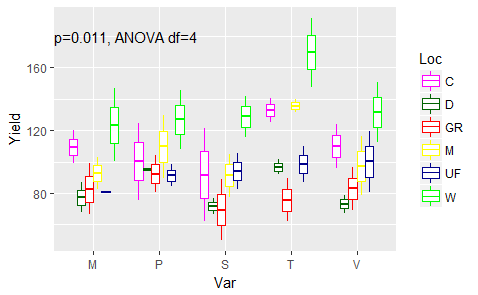
\includegraphics[width=\textwidth]{Figures/message4c}
	\end{center}
    \end{column}
    
    \begin{column}{0.5\textwidth}
    \begin{block}{Controlling for other sources of variation:}
      \begin{itemize}
	\item Control for year = compare yield WITHIN years and combine these
	\item Control for location = compare yield WITHIN locations and combine these
      \end{itemize}
      \end{block}
      \tiny Acknowledgements: MASS R-package
    \end{column}
  \end{columns}
   
\end{frame}
%%%%%%%%%%%


\begin{frame}{Message 4: Knowing how to combine information across subgroups  can improve inference}
 
  \begin{columns}
    \begin{column}{0.5\textwidth}
	\begin{center}
	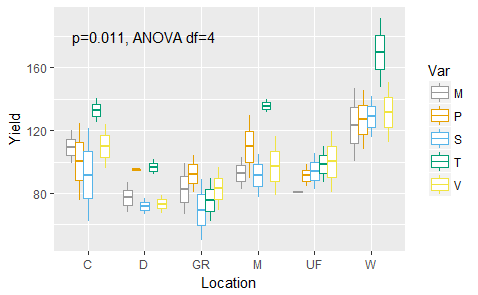
\includegraphics[width=\textwidth]{Figures/message4d}
	\end{center}
    \end{column}
    
    \begin{column}{0.5\textwidth}
    \begin{block}{Controlling for other sources of variation:}
      \begin{itemize}
	\item Control for year = compare yield WITHIN years and combine these
	\item Control for location = compare yield WITHIN locations and combine these
      \end{itemize}
      \end{block}
      \tiny Acknowledgements: MASS R-package
    \end{column}
  \end{columns}
   
\end{frame}
%%%%%%%%%%%


\end{document}
